%!TEX root = main.tex
\label{cap:sec2}
% What relevant differences in security performance does your metric reveal
%ToDo : cite owr first article
In this section we analize the output of the metrics proposed in~\cite{owr_article}. Based on this output we compare the performance of the distinct Autonomos Systems (AS) owners. We detail how the security performance can me compared using applying the metrics to a subset of the the problem owners i.e. ISPs in China.
% consider costumer, address space and services



\subsection{BN propagation}
It measures the number new IPs where the BNI attempts are being performed. It is useful to see the aggregate growth of the BN, and to help to infer a BNI rate.
This metric can be used to measure the evolution of the botnet in side a network. Since each ISP know the number of clients this metric can be normalized using this value. If an external party would like to compute and compare its perfromance using this metric, the normalization can be performed using the number of IP available addresses.

\subsection{BNI attempts}
It measures the number of attacks executed daily. We will use this data to analyze the BN activity. This metric could be useful to measure the effectiveness of mitigating controls. To analyze the security performance of the problem owner, we compare the activity comming from ISP networks and the activity comming from other service providers such as cloud providers and hosting providers. As we can see in figure~\ref{fig:as_day} the majority of the activity is comming form ASs which belongs several ISP, however, as we can see in the before mentioned figure, the service providers also are suffering a misuse of their resourses.

In figure~\ref{fig:isp_day} we show the attemts to infect the ellastichoney honeypot that are coming form the top 10 most active AS that belong to ISPs.As we see the more infected ISP is Chinanet but within its network the AS called Chinanet-js, located in the province of Zhejiang. This metric is aimed to be used by the problem owners, since further normalization is needed to get more accurate information, i.e. the market penetration per ISP per region.
% Overal growth (per network ?)
% Total cost


\begin{figure}[h]
     \caption{Attacks per day in diferent AS of the ISPs }
     \label{fig:isp_day}
    \centering
    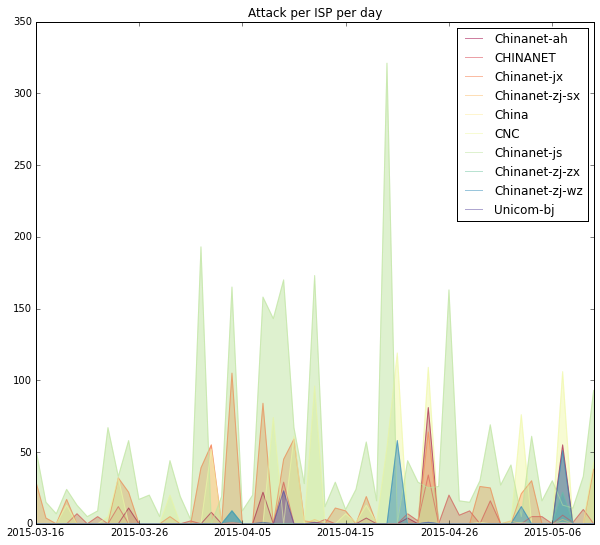
\includegraphics[width=\linewidth]{images/isp_legend_area}
\end{figure}


\begin{figure}[h]
    \caption{Activity coming from ISPs and other service providers}
    \label{fig:as_day}
    \centering
    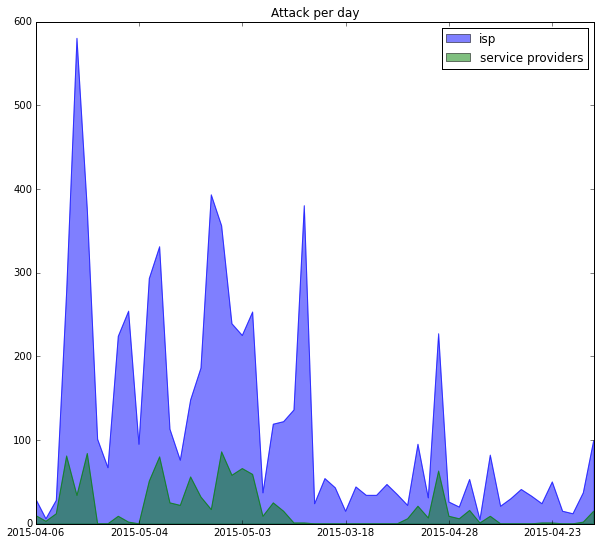
\includegraphics[width=\linewidth]{images/isp_no_isp_area}
\end{figure}
% % Infection ratio between net owners
